% Options for packages loaded elsewhere
% Options for packages loaded elsewhere
\PassOptionsToPackage{unicode}{hyperref}
\PassOptionsToPackage{hyphens}{url}
\PassOptionsToPackage{dvipsnames,svgnames,x11names}{xcolor}
%
\documentclass[
  letterpaper,
  DIV=11,
  numbers=noendperiod]{scrartcl}
\usepackage{xcolor}
\usepackage{amsmath,amssymb}
\setcounter{secnumdepth}{5}
\usepackage{iftex}
\ifPDFTeX
  \usepackage[T1]{fontenc}
  \usepackage[utf8]{inputenc}
  \usepackage{textcomp} % provide euro and other symbols
\else % if luatex or xetex
  \usepackage{unicode-math} % this also loads fontspec
  \defaultfontfeatures{Scale=MatchLowercase}
  \defaultfontfeatures[\rmfamily]{Ligatures=TeX,Scale=1}
\fi
\usepackage{lmodern}
\ifPDFTeX\else
  % xetex/luatex font selection
\fi
% Use upquote if available, for straight quotes in verbatim environments
\IfFileExists{upquote.sty}{\usepackage{upquote}}{}
\IfFileExists{microtype.sty}{% use microtype if available
  \usepackage[]{microtype}
  \UseMicrotypeSet[protrusion]{basicmath} % disable protrusion for tt fonts
}{}
\makeatletter
\@ifundefined{KOMAClassName}{% if non-KOMA class
  \IfFileExists{parskip.sty}{%
    \usepackage{parskip}
  }{% else
    \setlength{\parindent}{0pt}
    \setlength{\parskip}{6pt plus 2pt minus 1pt}}
}{% if KOMA class
  \KOMAoptions{parskip=half}}
\makeatother
% Make \paragraph and \subparagraph free-standing
\makeatletter
\ifx\paragraph\undefined\else
  \let\oldparagraph\paragraph
  \renewcommand{\paragraph}{
    \@ifstar
      \xxxParagraphStar
      \xxxParagraphNoStar
  }
  \newcommand{\xxxParagraphStar}[1]{\oldparagraph*{#1}\mbox{}}
  \newcommand{\xxxParagraphNoStar}[1]{\oldparagraph{#1}\mbox{}}
\fi
\ifx\subparagraph\undefined\else
  \let\oldsubparagraph\subparagraph
  \renewcommand{\subparagraph}{
    \@ifstar
      \xxxSubParagraphStar
      \xxxSubParagraphNoStar
  }
  \newcommand{\xxxSubParagraphStar}[1]{\oldsubparagraph*{#1}\mbox{}}
  \newcommand{\xxxSubParagraphNoStar}[1]{\oldsubparagraph{#1}\mbox{}}
\fi
\makeatother

\usepackage{color}
\usepackage{fancyvrb}
\newcommand{\VerbBar}{|}
\newcommand{\VERB}{\Verb[commandchars=\\\{\}]}
\DefineVerbatimEnvironment{Highlighting}{Verbatim}{commandchars=\\\{\}}
% Add ',fontsize=\small' for more characters per line
\usepackage{framed}
\definecolor{shadecolor}{RGB}{241,243,245}
\newenvironment{Shaded}{\begin{snugshade}}{\end{snugshade}}
\newcommand{\AlertTok}[1]{\textcolor[rgb]{0.68,0.00,0.00}{#1}}
\newcommand{\AnnotationTok}[1]{\textcolor[rgb]{0.37,0.37,0.37}{#1}}
\newcommand{\AttributeTok}[1]{\textcolor[rgb]{0.40,0.45,0.13}{#1}}
\newcommand{\BaseNTok}[1]{\textcolor[rgb]{0.68,0.00,0.00}{#1}}
\newcommand{\BuiltInTok}[1]{\textcolor[rgb]{0.00,0.23,0.31}{#1}}
\newcommand{\CharTok}[1]{\textcolor[rgb]{0.13,0.47,0.30}{#1}}
\newcommand{\CommentTok}[1]{\textcolor[rgb]{0.37,0.37,0.37}{#1}}
\newcommand{\CommentVarTok}[1]{\textcolor[rgb]{0.37,0.37,0.37}{\textit{#1}}}
\newcommand{\ConstantTok}[1]{\textcolor[rgb]{0.56,0.35,0.01}{#1}}
\newcommand{\ControlFlowTok}[1]{\textcolor[rgb]{0.00,0.23,0.31}{\textbf{#1}}}
\newcommand{\DataTypeTok}[1]{\textcolor[rgb]{0.68,0.00,0.00}{#1}}
\newcommand{\DecValTok}[1]{\textcolor[rgb]{0.68,0.00,0.00}{#1}}
\newcommand{\DocumentationTok}[1]{\textcolor[rgb]{0.37,0.37,0.37}{\textit{#1}}}
\newcommand{\ErrorTok}[1]{\textcolor[rgb]{0.68,0.00,0.00}{#1}}
\newcommand{\ExtensionTok}[1]{\textcolor[rgb]{0.00,0.23,0.31}{#1}}
\newcommand{\FloatTok}[1]{\textcolor[rgb]{0.68,0.00,0.00}{#1}}
\newcommand{\FunctionTok}[1]{\textcolor[rgb]{0.28,0.35,0.67}{#1}}
\newcommand{\ImportTok}[1]{\textcolor[rgb]{0.00,0.46,0.62}{#1}}
\newcommand{\InformationTok}[1]{\textcolor[rgb]{0.37,0.37,0.37}{#1}}
\newcommand{\KeywordTok}[1]{\textcolor[rgb]{0.00,0.23,0.31}{\textbf{#1}}}
\newcommand{\NormalTok}[1]{\textcolor[rgb]{0.00,0.23,0.31}{#1}}
\newcommand{\OperatorTok}[1]{\textcolor[rgb]{0.37,0.37,0.37}{#1}}
\newcommand{\OtherTok}[1]{\textcolor[rgb]{0.00,0.23,0.31}{#1}}
\newcommand{\PreprocessorTok}[1]{\textcolor[rgb]{0.68,0.00,0.00}{#1}}
\newcommand{\RegionMarkerTok}[1]{\textcolor[rgb]{0.00,0.23,0.31}{#1}}
\newcommand{\SpecialCharTok}[1]{\textcolor[rgb]{0.37,0.37,0.37}{#1}}
\newcommand{\SpecialStringTok}[1]{\textcolor[rgb]{0.13,0.47,0.30}{#1}}
\newcommand{\StringTok}[1]{\textcolor[rgb]{0.13,0.47,0.30}{#1}}
\newcommand{\VariableTok}[1]{\textcolor[rgb]{0.07,0.07,0.07}{#1}}
\newcommand{\VerbatimStringTok}[1]{\textcolor[rgb]{0.13,0.47,0.30}{#1}}
\newcommand{\WarningTok}[1]{\textcolor[rgb]{0.37,0.37,0.37}{\textit{#1}}}

\usepackage{longtable,booktabs,array}
\newcounter{none} % for unnumbered tables
\usepackage{calc} % for calculating minipage widths
% Correct order of tables after \paragraph or \subparagraph
\usepackage{etoolbox}
\makeatletter
\patchcmd\longtable{\par}{\if@noskipsec\mbox{}\fi\par}{}{}
\makeatother
% Allow footnotes in longtable head/foot
\IfFileExists{footnotehyper.sty}{\usepackage{footnotehyper}}{\usepackage{footnote}}
\makesavenoteenv{longtable}
\usepackage{graphicx}
\makeatletter
\newsavebox\pandoc@box
\newcommand*\pandocbounded[1]{% scales image to fit in text height/width
  \sbox\pandoc@box{#1}%
  \Gscale@div\@tempa{\textheight}{\dimexpr\ht\pandoc@box+\dp\pandoc@box\relax}%
  \Gscale@div\@tempb{\linewidth}{\wd\pandoc@box}%
  \ifdim\@tempb\p@<\@tempa\p@\let\@tempa\@tempb\fi% select the smaller of both
  \ifdim\@tempa\p@<\p@\scalebox{\@tempa}{\usebox\pandoc@box}%
  \else\usebox{\pandoc@box}%
  \fi%
}
% Set default figure placement to htbp
\def\fps@figure{htbp}
\makeatother





\setlength{\emergencystretch}{3em} % prevent overfull lines

\providecommand{\tightlist}{%
  \setlength{\itemsep}{0pt}\setlength{\parskip}{0pt}}



 


\KOMAoption{captions}{tableheading}
\makeatletter
\@ifpackageloaded{tcolorbox}{}{\usepackage[skins,breakable]{tcolorbox}}
\@ifpackageloaded{fontawesome5}{}{\usepackage{fontawesome5}}
\definecolor{quarto-callout-color}{HTML}{909090}
\definecolor{quarto-callout-note-color}{HTML}{0758E5}
\definecolor{quarto-callout-important-color}{HTML}{CC1914}
\definecolor{quarto-callout-warning-color}{HTML}{EB9113}
\definecolor{quarto-callout-tip-color}{HTML}{00A047}
\definecolor{quarto-callout-caution-color}{HTML}{FC5300}
\definecolor{quarto-callout-color-frame}{HTML}{acacac}
\definecolor{quarto-callout-note-color-frame}{HTML}{4582ec}
\definecolor{quarto-callout-important-color-frame}{HTML}{d9534f}
\definecolor{quarto-callout-warning-color-frame}{HTML}{f0ad4e}
\definecolor{quarto-callout-tip-color-frame}{HTML}{02b875}
\definecolor{quarto-callout-caution-color-frame}{HTML}{fd7e14}
\makeatother
\makeatletter
\@ifpackageloaded{caption}{}{\usepackage{caption}}
\AtBeginDocument{%
\ifdefined\contentsname
  \renewcommand*\contentsname{Table of contents}
\else
  \newcommand\contentsname{Table of contents}
\fi
\ifdefined\listfigurename
  \renewcommand*\listfigurename{List of Figures}
\else
  \newcommand\listfigurename{List of Figures}
\fi
\ifdefined\listtablename
  \renewcommand*\listtablename{List of Tables}
\else
  \newcommand\listtablename{List of Tables}
\fi
\ifdefined\figurename
  \renewcommand*\figurename{Figure}
\else
  \newcommand\figurename{Figure}
\fi
\ifdefined\tablename
  \renewcommand*\tablename{Table}
\else
  \newcommand\tablename{Table}
\fi
}
\@ifpackageloaded{float}{}{\usepackage{float}}
\floatstyle{ruled}
\@ifundefined{c@chapter}{\newfloat{codelisting}{h}{lop}}{\newfloat{codelisting}{h}{lop}[chapter]}
\floatname{codelisting}{Listing}
\newcommand*\listoflistings{\listof{codelisting}{List of Listings}}
\makeatother
\makeatletter
\makeatother
\makeatletter
\@ifpackageloaded{caption}{}{\usepackage{caption}}
\@ifpackageloaded{subcaption}{}{\usepackage{subcaption}}
\makeatother
\usepackage{bookmark}
\IfFileExists{xurl.sty}{\usepackage{xurl}}{} % add URL line breaks if available
\urlstyle{same}
% fallback for those not using the hyperref driver hyperxmp:
\makeatletter
\@ifundefined{xmpquote}{\newcommand{\xmpquote}[1]{#1}}{}
\makeatother
\hypersetup{
  pdftitle={Course Introduction},
  pdfauthor={Paolo Bosetti},
  colorlinks=true,
  linkcolor={blue},
  filecolor={Maroon},
  citecolor={Blue},
  urlcolor={Blue},
  pdfcreator={LaTeX via pandoc}}


\title{Course Introduction}
\usepackage{etoolbox}
\makeatletter
\providecommand{\subtitle}[1]{% add subtitle to \maketitle
  \apptocmd{\@title}{\par {\large #1 \par}}{}{}
}
\makeatother
\subtitle{Digital Manufacturing\\

\includegraphics[width=\linewidth,height=0.3125in,keepaspectratio]{images/by-nc-sa.png}}
\author{Paolo Bosetti}
\date{\emph{Updated:} 14/10/2026}
\begin{document}
\maketitle

\renewcommand*\contentsname{Table of contents}
{
\setcounter{tocdepth}{3}
\tableofcontents
}

\begin{Shaded}
\begin{Highlighting}[]
\FunctionTok{options}\NormalTok{(}\AttributeTok{width =} \DecValTok{60}\NormalTok{)}
\FunctionTok{set.seed}\NormalTok{(}\DecValTok{0}\NormalTok{)}
\end{Highlighting}
\end{Shaded}

\section{Digital Manufacturing}\label{digital-manufacturing}

\begin{itemize}
\tightlist
\item
  DM is the evolution of manufacturing, where an integrated approach is
  centered around a computer system
\item
  Evolution: purely mechanical machinery ➡︎ CNC machines ➡︎ systems of
  computer-controlled machines
\item
  DM goes within the framework of Industry 4.0
\item
  Industry 4.0 is the 4th industrial revolution
\end{itemize}

\section{Evolution of manufacturing}\label{evolution-of-manufacturing}

\begin{figure}[H]

{\centering 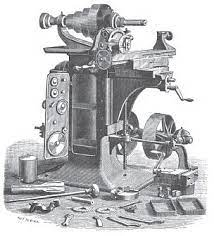
\includegraphics[width=\linewidth,height=1.97917in,keepaspectratio]{images/milling.jpg}

}

\caption{Milling machine}

\end{figure}%

\begin{figure}[H]

{\centering 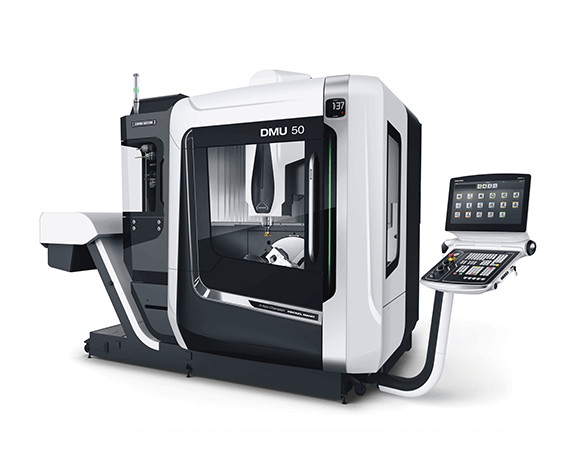
\includegraphics[width=\linewidth,height=1.97917in,keepaspectratio]{images/cnc.png}

}

\caption{CNC milling center}

\end{figure}%

\begin{figure}[H]

{\centering 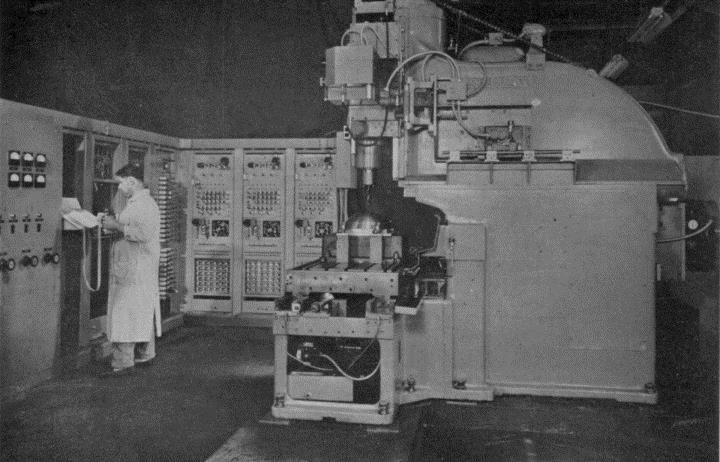
\includegraphics[width=\linewidth,height=1.97917in,keepaspectratio]{images/first-nc.png}

}

\caption{1st NC machine tool (MIT, 1952)}

\end{figure}%

\begin{figure}[H]

{\centering 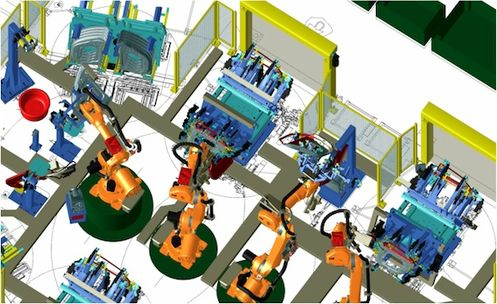
\includegraphics[width=\linewidth,height=1.97917in,keepaspectratio]{images/dm-plant.jpg}

}

\caption{DM plant}

\end{figure}%

\section{Industry 4.0}\label{industry-4.0}

The term is a \textbf{marketing slogan} for the 4th industrial
revolution, which is the \textbf{digitalization of manufacturing}. It
was coined in Germany in 2011, and it is now a worldwide concept.

\begin{itemize}
\tightlist
\item
  \textbf{Motivation} --- reaction from EU and USA to 2008 economical
  crisis
\item
  \textbf{Name origin} --- 2011 Hannover Messe (Angela Merkel)
\end{itemize}

\begin{itemize}
\tightlist
\item
  Hannover Messe 2013 --- presentation of \textbf{final report} of the
  \emph{Industrie 4.0} committee, \textbf{tasked by German government}
  in 2011:

  \begin{itemize}
  \tightlist
  \item
    Design principles
  \item
    Challenges
  \item
    Impacts
  \end{itemize}
\end{itemize}

\begin{center}
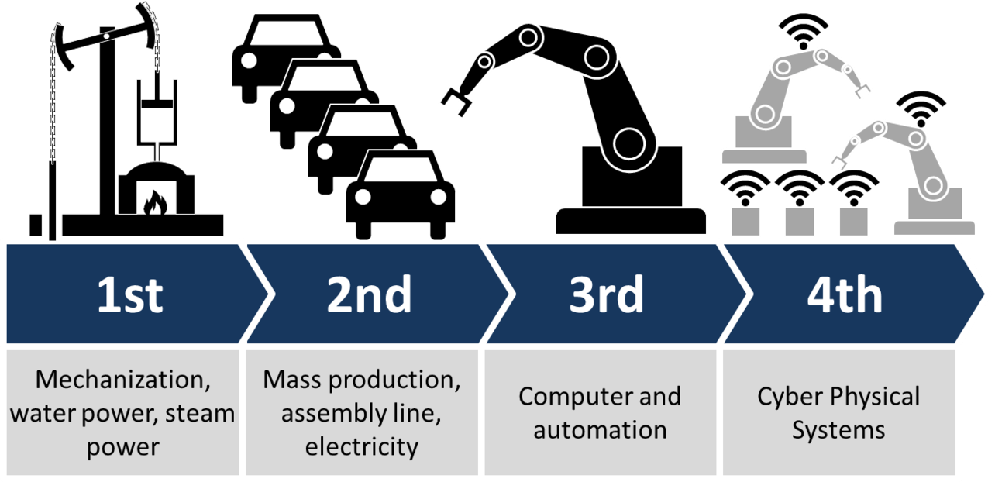
\includegraphics[width=\linewidth,height=3.125in,keepaspectratio]{images/industry40.png}
\end{center}

\section{Previous industrial
revolutions}\label{previous-industrial-revolutions}

\textbf{First Industrial Revolution}

\begin{figure}[H]

{\centering 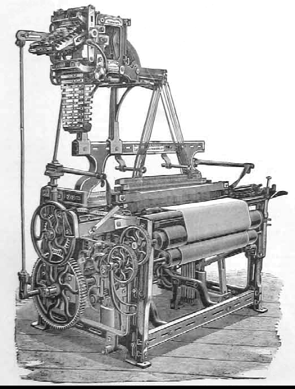
\includegraphics[width=0.9\linewidth,height=\textheight,keepaspectratio]{images/loom.png}

}

\caption{Mechanical loom, E. Cartwright, \textbf{1784}}

\end{figure}%

\textbf{Second Industrial Revolution}

\begin{figure}[H]

{\centering 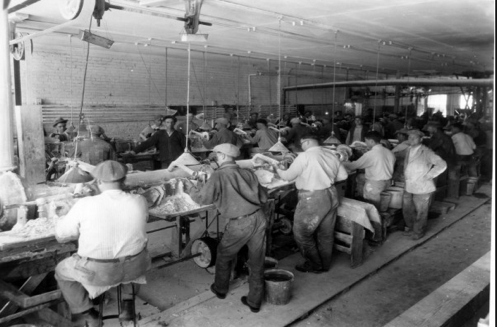
\includegraphics[width=0.65\linewidth,height=\textheight,keepaspectratio]{images/conveyor-cincinnati.png}

}

\caption{Conveyor belt, Cincinnati Slaughterhouse, \textbf{1870}}

\end{figure}%

\begin{figure}[H]

{\centering 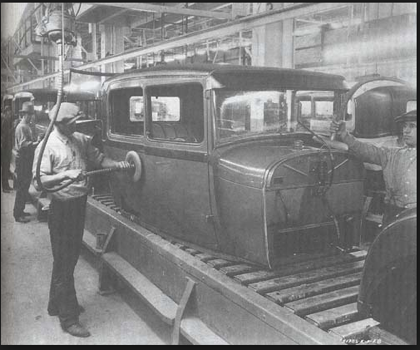
\includegraphics[width=0.65\linewidth,height=\textheight,keepaspectratio]{images/conveyor-ford.png}

}

\caption{Conveyor belt, Ford Motor Company, \textbf{1913}}

\end{figure}%

\textbf{Third Industrial Revolution}

\begin{figure}[H]

{\centering 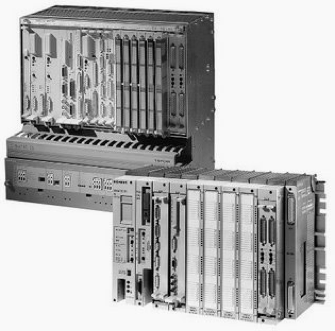
\includegraphics[width=0.9\linewidth,height=\textheight,keepaspectratio]{images/plc.png}

}

\caption{PLC, Modicon 084, \textbf{1969}}

\end{figure}%

\section{Industry 4.0}\label{industry-4.0-1}

\textbf{Objectives:}

\begin{itemize}
\tightlist
\item
  Re-shoring of added value in western countries
\item
  Sustain salaries of working- and middle-class
\item
  Sustain e-commerce
\item
  Mass customization (added value shifts from manufacturing to design)
\item
  Time compression (life cycle of a car from 5 to 2 years)
\end{itemize}

\section{Industry 4.0}\label{industry-4.0-2}

\textbf{Design principles:}

\begin{itemize}
\tightlist
\item
  Interoperability (IoT, IIoT, IoP)
\item
  Cyber-Physical Systems (CPS)
\item
  Information transparency: public, open protocols; digital twins
\item
  Self-support and in-line help to operators
\item
  Decision de-centralization: autonomy, stratification, prioritization
\end{itemize}

\section{Industry 4.0}\label{industry-4.0-3}

\begin{longtable}[]{@{}
  >{\raggedright\arraybackslash}p{(\linewidth - 4\tabcolsep) * \real{0.1429}}
  >{\raggedright\arraybackslash}p{(\linewidth - 4\tabcolsep) * \real{0.1429}}
  >{\raggedright\arraybackslash}p{(\linewidth - 4\tabcolsep) * \real{0.7143}}@{}}
\caption{Akin to the \emph{Yardstick of Automation} (Amber \& Amber,
1962)}\tabularnewline
\toprule\noalign{}
\begin{minipage}[b]{\linewidth}\raggedright
Order
\end{minipage} & \begin{minipage}[b]{\linewidth}\raggedright
Human attribute
\end{minipage} & \begin{minipage}[b]{\linewidth}\raggedright
Example
\end{minipage} \\
\midrule\noalign{}
\endfirsthead
\toprule\noalign{}
\begin{minipage}[b]{\linewidth}\raggedright
Order
\end{minipage} & \begin{minipage}[b]{\linewidth}\raggedright
Human attribute
\end{minipage} & \begin{minipage}[b]{\linewidth}\raggedright
Example
\end{minipage} \\
\midrule\noalign{}
\endhead
\bottomrule\noalign{}
\endlastfoot
0 & None & Manual tools \\
1 & Energy & Powered machines and tools \\
2 & Dexterity & Single-cycle automatics (\emph{dexterity =
self-feeding}) \\
3 & Diligence & Repeats cycle; open-loop control \\
4 & Judgment & Closed loop; numerical control; self-measuring \\
5 & Evaluation & Computer control; model of process required for
automation \\
6 & Learning & Limited self-programming; some artificial intelligence \\
7 & Reasoning & Inductive reasoning (cause-effects) \\
8 & Creativity & Performs (original) design unaided \\
9 & Dominance & Machine is master (HAL 9000) \\
\end{longtable}

\section{Industry 4.0}\label{industry-4.0-4}

\textbf{Challenges:}

\begin{itemize}
\tightlist
\item
  Cybersecurity
\item
  Reliability and resiliency of M2M communication (bandwidth and
  latency)
\item
  Drop-in, plug-in approach on existing processes
\item
  Intellectual property (IP) protection
\item
  Reluctancy to change, operators re-training
\item
  Corporate IT
\item
  Initial loss of labor
\end{itemize}

\section{Industry 4.0}\label{industry-4.0-5}

\textbf{Impacts:}

\begin{itemize}
\tightlist
\item
  Servitization (from selling goods to selling services)
\item
  Productivity, and its resilience
\item
  Safety
\item
  Integrated design of product/process
\item
  Cost structure
\item
  Socio-economical factors
\item
  Big Data analytics
\end{itemize}

\section{Digital Manufacturing}\label{digital-manufacturing-1}

A set of core, \textbf{enabling technologies} are grounding I4.0 and DM:

\begin{itemize}
\tightlist
\item
  \textbf{Cyber-Physical Systems} (M2M connectivity): in short, they are
  mechatronic systems, i.e., mechanisms, whose actuators are controlled
  by a computer system based on output from sensors and logics provided
  by algorithms
\item
  CPSs provide the plant controller with information on its own status
\item
  \textbf{IIoT} (connectivity layer): \emph{Industrial Internet of
  Things}
\item
  Additive Manufacturing (dematerialization of design): paradigm of
  \textbf{fully digital manufacturing process}
\item
  \textbf{Machine Learning} and AI: strategy to further enhance the
  level of automation and enable autonomous decisions
\end{itemize}

\section{Digital Manufacturing}\label{digital-manufacturing-2}

\begin{itemize}
\tightlist
\item
  \textbf{Industrial Internet of Things (IIoT):} has to support
  communications among CPSs (M2M communication)
\item
  Every \textbf{device} is on the network: we have tens of billions of
  devices globally connected, and the number is growing fast
\item
  \textbf{Problem}: IP protocol: IPv4 has
  \(2^{32} \simeq 4.3 \times 10^9\) addresses
\item
  \textbf{Solutions}:

  \begin{itemize}
  \tightlist
  \item
    IPv6 has \(2^{128} \simeq 3.4 \times 10^{39}\) addresses, but IPv6
    adoption is slow because of the added costs and complexities
  \item
    \textbf{NAT}
    (\href{https://en.wikipedia.org/wiki/Network_address_translation}{\emph{Network
    Address Translation}}) keeps IPv4 and addresses exhaustion problem
    by allowing multiple devices to share a single public IP address
    behind a gateway
  \end{itemize}
\end{itemize}

\section{OSI Networking Model}\label{osi-networking-model}

\begin{itemize}
\tightlist
\item
  Networking stack: according to the Internet model, networking happens
  over a stack of 4 layers
\end{itemize}

\begin{itemize}
\tightlist
\item
  \textbf{Link layer} (L0): physical carrier (Ethernet Cable, WiFi, etc)
  and its protocol (MAC, 802.11, ARP, etc)
\item
  \textbf{Internet (or network) layer} (L1): IPv4, IPv6, ICMP
\item
  \textbf{Transport layer} (L2): TCP, UDP
\item
  \textbf{Application layer} (L3): HTTP, FTP, IMAP, LDAP, \ldots{}
\end{itemize}

\begin{figure}[H]

{\centering 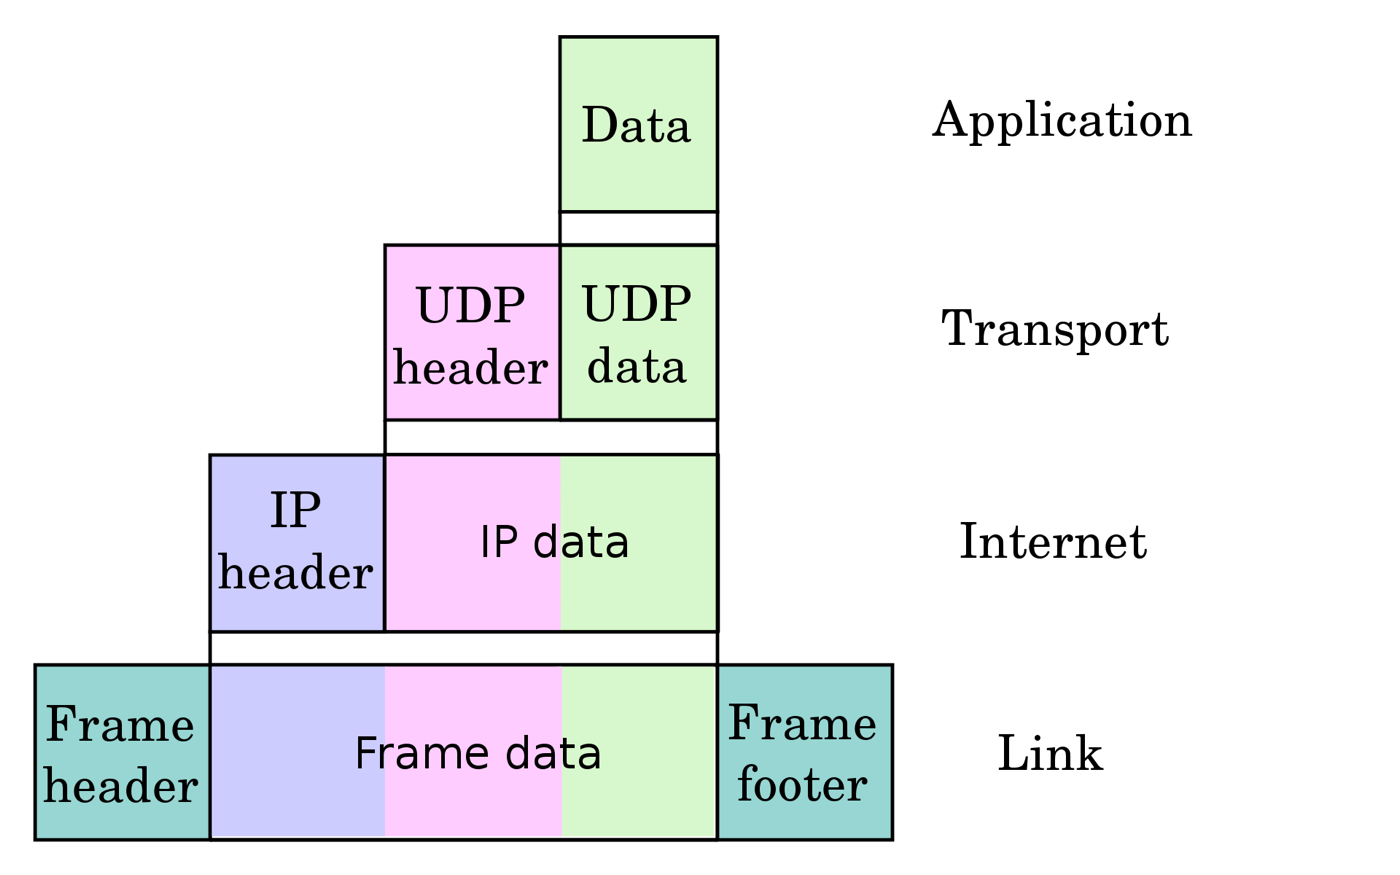
\includegraphics[width=\linewidth,height=2.91667in,keepaspectratio]{images/udp-encapsulation.png}

}

\caption{OSI layers}

\end{figure}%

\section{Digital Manufacturing}\label{digital-manufacturing-3}

\textbf{Industrial Internet of Things (IIoT):} has to support
communications among CPSs (M2M communication)

\begin{itemize}
\tightlist
\item
  \textbf{Level 0 protocols:} as fast as possible; currently introducing
  5G (wireless yet extra-low latency!)
\item
  \textbf{IP protocol (L1):} beside address space, IPv6 has other
  advantages (complex multicasting, autoconfiguration, IPsec). Its
  adoption is still slow, though
\item
  \textbf{Level 3 protocols:} moving from REST (HTTPS) to more
  lightweight \textbf{message queuing protocols} (MQTT, ZeroMQ, AMQP,
  OPC-UA)
\end{itemize}

\section{REST vs Message Queuing}\label{rest-vs-message-queuing}

\begin{itemize}
\tightlist
\item
  \textbf{RE}presentational \textbf{S}tate \textbf{T}ransfer: it is an
  IoT extension of HTTP
\item
  It is not ideal:

  \begin{itemize}
  \tightlist
  \item
    Verbose: large overhead
  \item
    Complex: \texttt{PUT/GET/POST/DELETE} verbs that make sense for IoP,
    but not for IoT
  \item
    Polling-based, event-based actions difficult to implement
  \item
    Point-to-point: \emph{n} clients to 1 server; routing a message
    between clients is difficult and not efficient
  \end{itemize}
\end{itemize}

\begin{center}
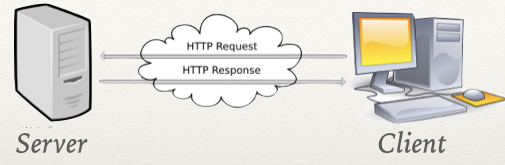
\includegraphics[width=\linewidth,height=1.77083in,keepaspectratio]{images/rest.png}
\end{center}

\section{HTTP overhead}\label{http-overhead}

Let's see a HTTP/TCP request/reply message exchange by capturing the
whole traffic with \href{https://www.wireshark.org/}{Wireshark}

\begin{itemize}
\tightlist
\item
  Request phrase: \texttt{GET\ /\ HTTP/1.1} (14 × 2 bytes)
\item
  The HTTP frame takes 153 bytes total
\item
  The full request stack takes 437 bytes for the \textbf{minimum
  request}
\end{itemize}

\begin{figure}[H]

{\centering 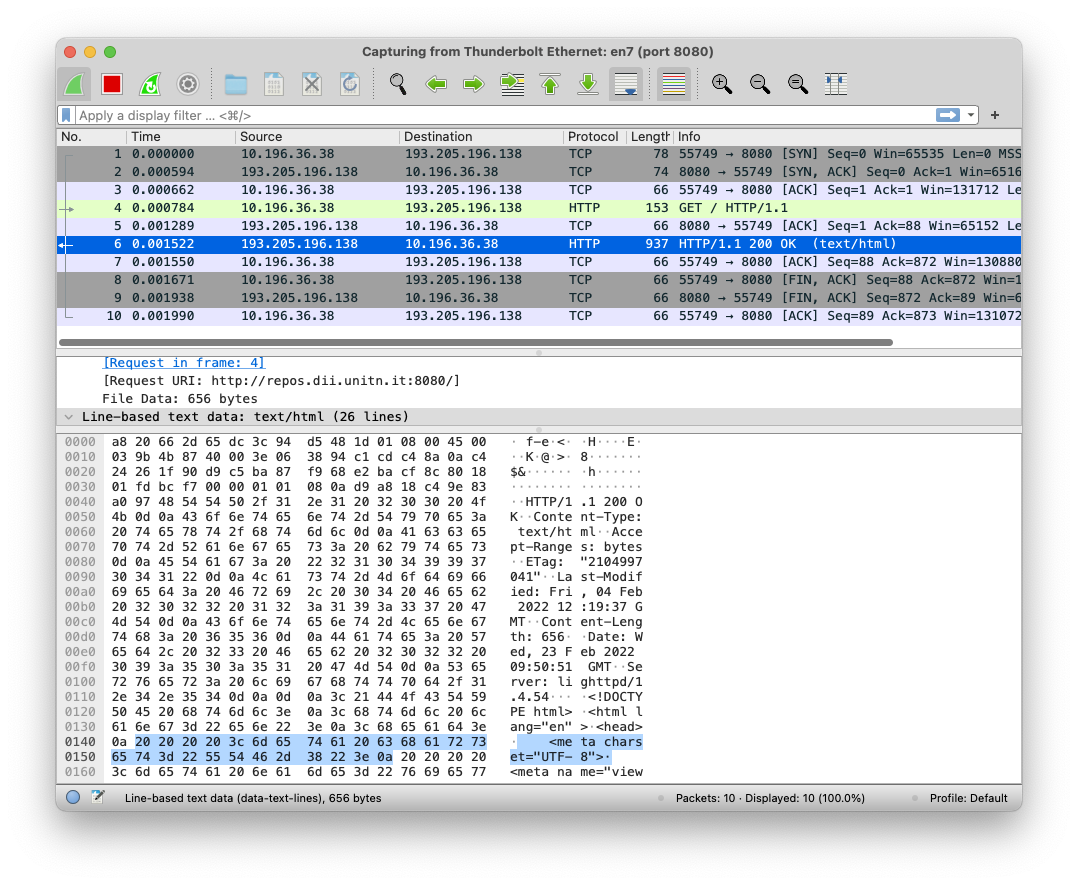
\includegraphics[width=\linewidth,height=4.89583in,keepaspectratio]{images/wireshark-1.png}

}

\caption{Wireshark capture}

\end{figure}%

\section{HTTP overhead}\label{http-overhead-1}

\begin{itemize}
\tightlist
\item
  Response phrase: 77 bytes + HTML
\item
  The whole HTTP frame takes 937 bytes (including 819 bytes of HTML)
\item
  The full response stack takes 1201 bytes, 382 bytes for a
  \textbf{blank page}
\end{itemize}

\begin{tcolorbox}[enhanced jigsaw, arc=.35mm, bottomrule=.15mm, bottomtitle=1mm, breakable, colback=white, colbacktitle=quarto-callout-warning-color!10!white, colframe=quarto-callout-warning-color-frame, coltitle=black, left=2mm, leftrule=.75mm, opacityback=0, opacitybacktitle=0.6, rightrule=.15mm, title=\textcolor{quarto-callout-warning-color}{\faExclamationTriangle}\hspace{0.5em}{Overhead}, titlerule=0mm, toprule=.15mm, toptitle=1mm]

This is a \textbf{huge overhead} for a simple request/reply message
exchange, and it is not acceptable for IoT communications, because it
adds both bandwidth \textbf{and} latency

\end{tcolorbox}

\begin{figure}[H]

{\centering 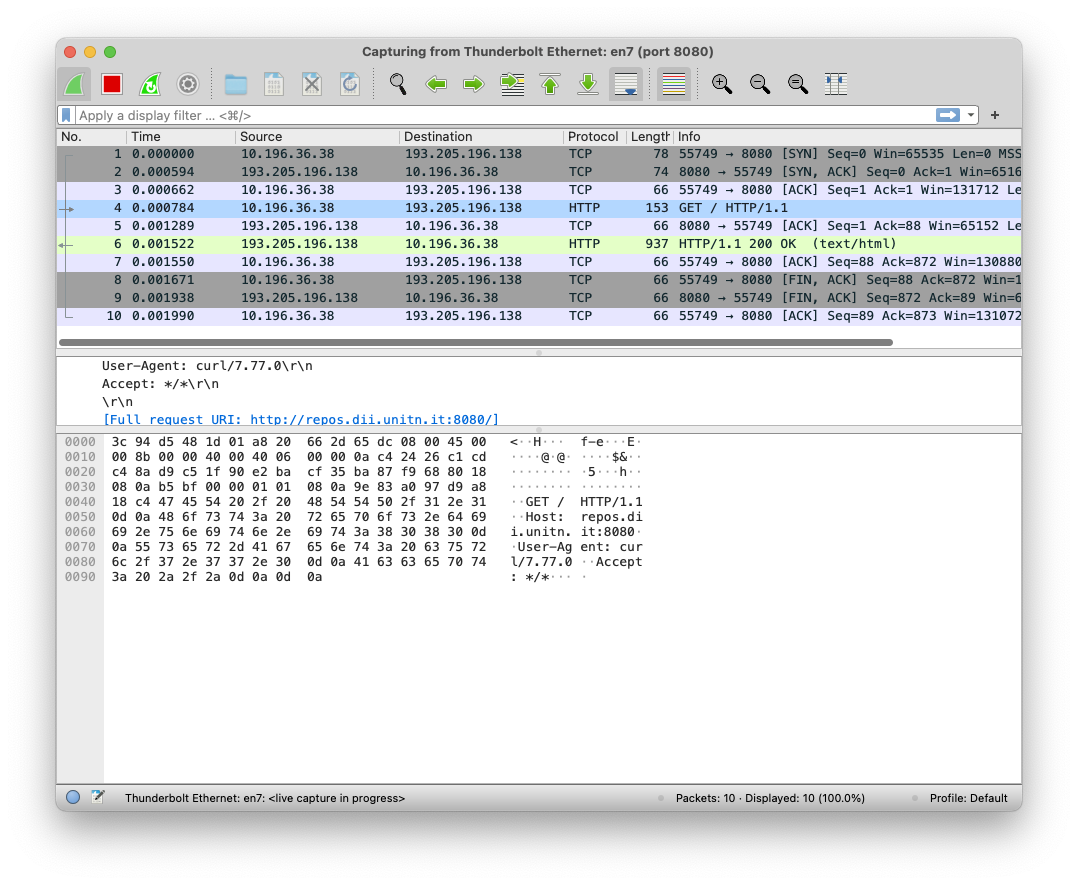
\includegraphics[width=\linewidth,height=4.89583in,keepaspectratio]{images/wireshark-2.png}

}

\caption{Wireshark capture}

\end{figure}%

\section{How to reduce overhead}\label{how-to-reduce-overhead}

\begin{itemize}
\tightlist
\item
  Reliability and robustness are very important for \textbf{IoP}
  communications: variety of web servers, web browsers and document
  formats, and the web must ``just work''
\item
  They are also important in \textbf{IoT} (because \emph{things} must do
  their tasks) but we can enforce standards and minimize possible
  sources of unexpected conditions
\end{itemize}

Overhead can be reduced by:

\begin{itemize}
\tightlist
\item
  Simpler transport layer (L2) protocol: UDP has no SYN/ACK/FIN frames
  (but no confirmation of delivery!)
\item
  Simpler application layer (L3) protocols, where the data frame is as
  naked as possible
\item
  Trading reliability and robustness for bandwidth and latency
\end{itemize}

\section{REST vs Message Queuing}\label{rest-vs-message-queuing-1}

\begin{itemize}
\tightlist
\item
  IoT messages are typically smaller but much more frequent than IoP
  messages, and \textbf{may need to follow routes more complex than
  n-to-1} (client\textbf{s}--server)

  \begin{itemize}
  \tightlist
  \item
    Need to minimize overhead
  \item
    Need to support flexible topologies
  \end{itemize}
\item
  Message Queuing protocols (like MQTT and ZeroMQ)
\end{itemize}

\includegraphics[width=5.03in,height=3.98in]{0-intro_files/figure-latex/mermaid-figure-1.png}

\section{REST vs Message Queuing}\label{rest-vs-message-queuing-2}

\begin{center}
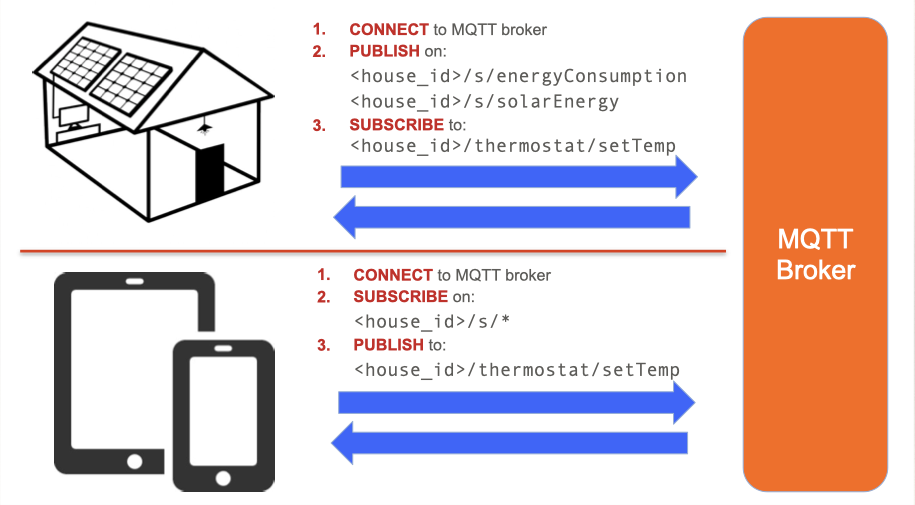
\includegraphics[width=\linewidth,height=5.20833in,keepaspectratio]{images/mqtt-broker.png}
\end{center}

\section{Digital Manufacturing}\label{digital-manufacturing-4}

It is the effort of moving all information flow from the design phase to
the manufacturing phase into a digital (paperless) workflow, with the
final goal of {minimizing human effort and intervention} (automation)

\begin{itemize}
\tightlist
\item
  \textbf{Conventional machining:} Designer ➡︎ Drawings/models ➡︎ CAM
  operator ➡︎ part-program ➡︎ CNC machine tool
\item
  \textbf{Additive Manufacturing:} Designer ➡︎ Machine tool (like a
  printer)
\item
  Entirely digital workflow, minimal human intervention
\item
  Support for \textbf{Machine Learning} and Artificial Intelligence:

  \begin{itemize}
  \tightlist
  \item
    Classification of operating conditions
  \item
    Autonomous and de-centralized decision making
  \item
    Level 7 automation on Amber \& Amber's scale
  \end{itemize}
\end{itemize}

\section{Course Matter}\label{course-matter}

\begin{enumerate}
\def\labelenumi{\arabic{enumi}.}
\tightlist
\item
  Overview of manufacturing processes, machine architectures, control
  algorithms
\item
  Development of a CNC kernel (motion planner and controller)
\item
  Interfacing the CNC kernel with a digital twin (Simulink model) and a
  3D viewer, using an IoT framework
\end{enumerate}

\begin{figure}[H]

{\centering 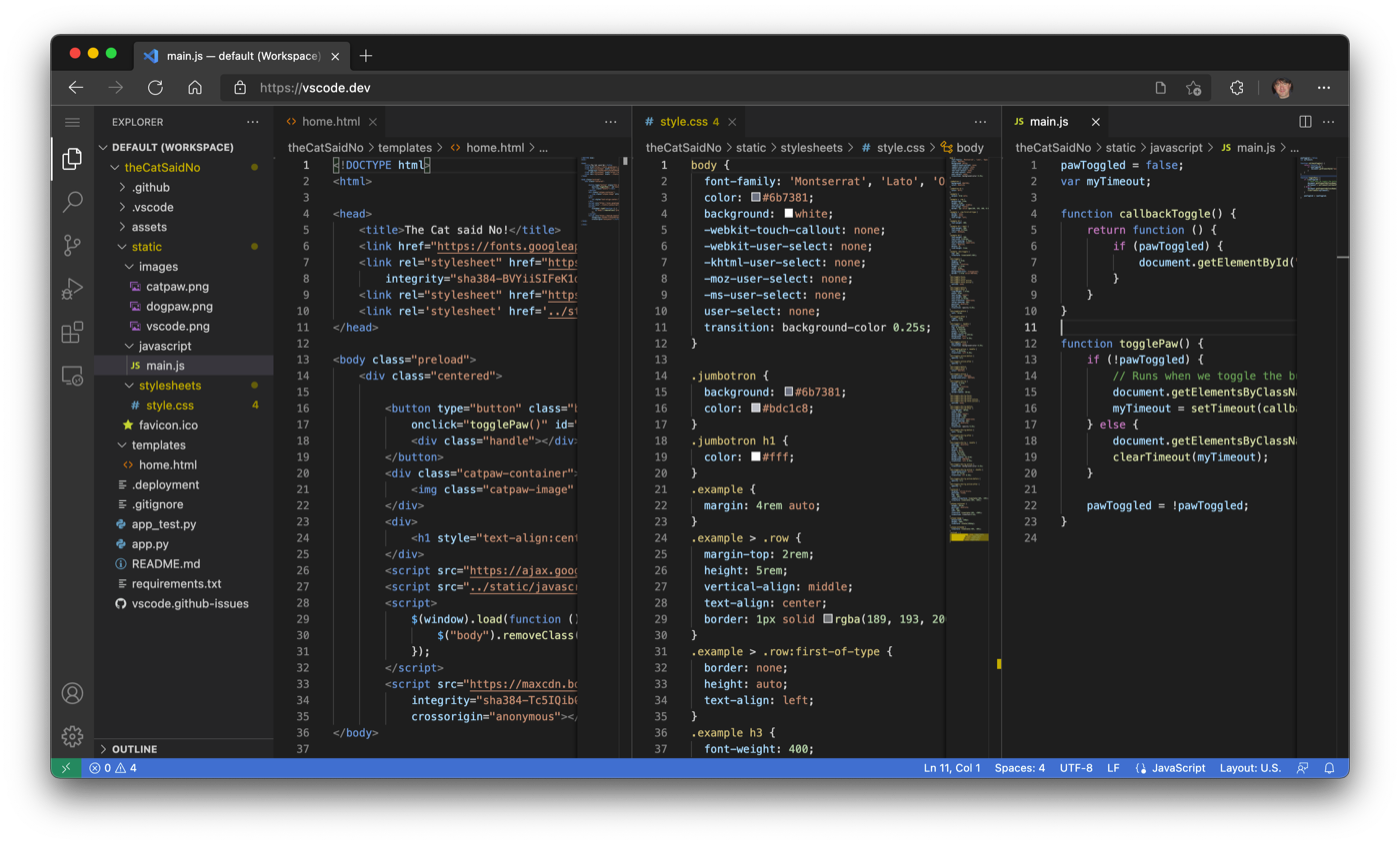
\includegraphics[width=\linewidth,height=3.125in,keepaspectratio]{images/vscode.png}

}

\caption{C++ development and testing}

\end{figure}%

\begin{figure}[H]

{\centering 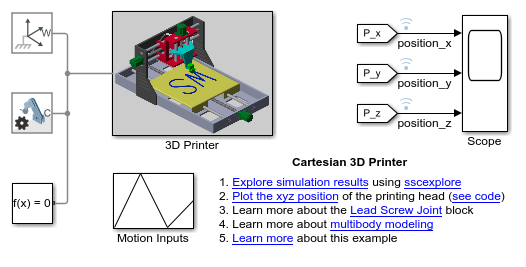
\includegraphics[width=\linewidth,height=3.125in,keepaspectratio]{images/simulink.png}

}

\caption{CPS simulation (Digital Twin)}

\end{figure}%

\begin{figure}[H]

{\centering 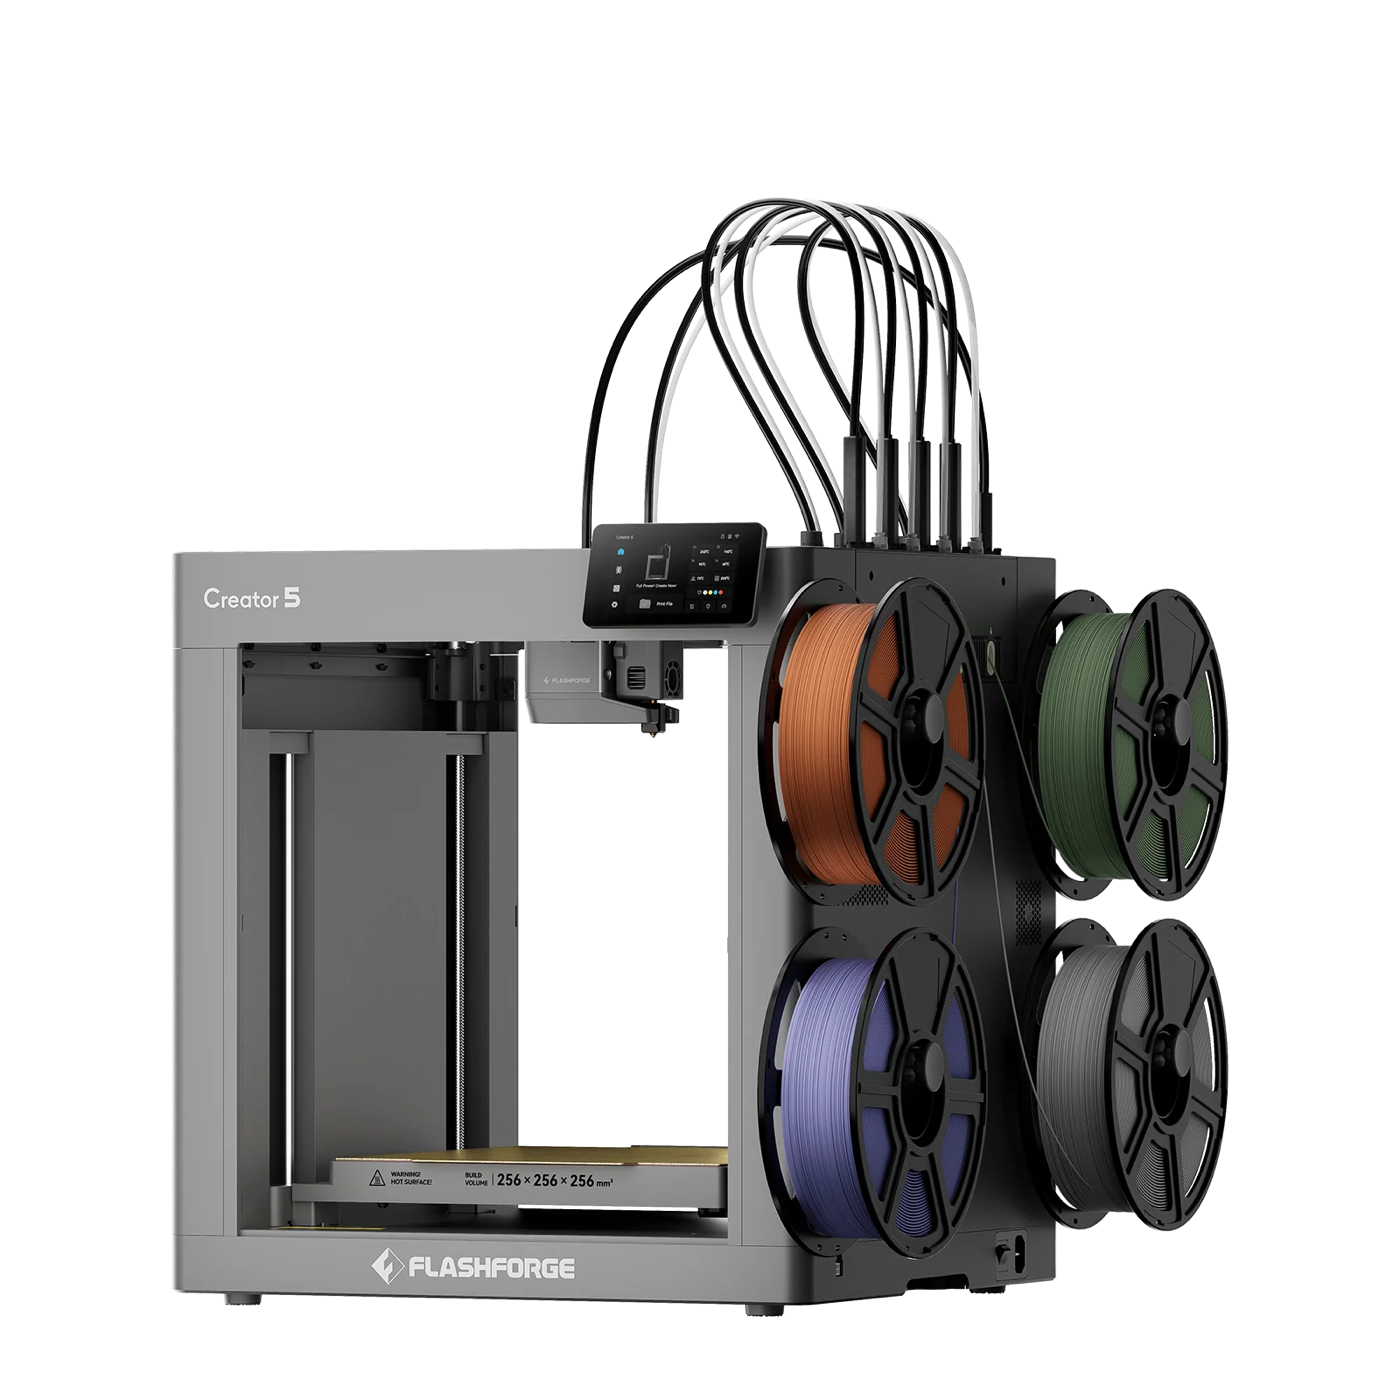
\includegraphics[width=\linewidth,height=3.125in,keepaspectratio]{images/printer.png}

}

\caption{3D printer/3D viewer}

\end{figure}%

\section{Tools}\label{tools}

\begin{itemize}
\tightlist
\item
  \textbf{Programming in C++}: high performance, general purpose
  language, suitable for real-time systems (controllers), more complex
  to learn than C (bigger) but more abstract (does not need
  understanding of hardware)
\item
  \textbf{GNU-Unix toolchain} (much more common than Windows in
  automation)

  \begin{itemize}
  \tightlist
  \item
    Linux exposed via WSL in Windows (MacOS is UNIX already)
  \item
    And/or custom machine simulator (faster)
  \end{itemize}
\item
  Code will be developed in class and made available on
  \url{https://github.com/pbosetti/cncpp}
\item
  Reference \textbf{IoT framework} is
  \href{https://mads-net.github.io}{MADS}
\end{itemize}

\section{Teaching Material}\label{teaching-material}

\begin{itemize}
\tightlist
\item
  All teaching materials are provided via Moodle
\item
  Software will be made available on GitHub platform
\item
  Reference textbook is \emph{Manufacturing Automation}, by Y. Altintas
  (2000), available @BUM (2 copies)
\end{itemize}

\begin{figure}[H]

{\centering 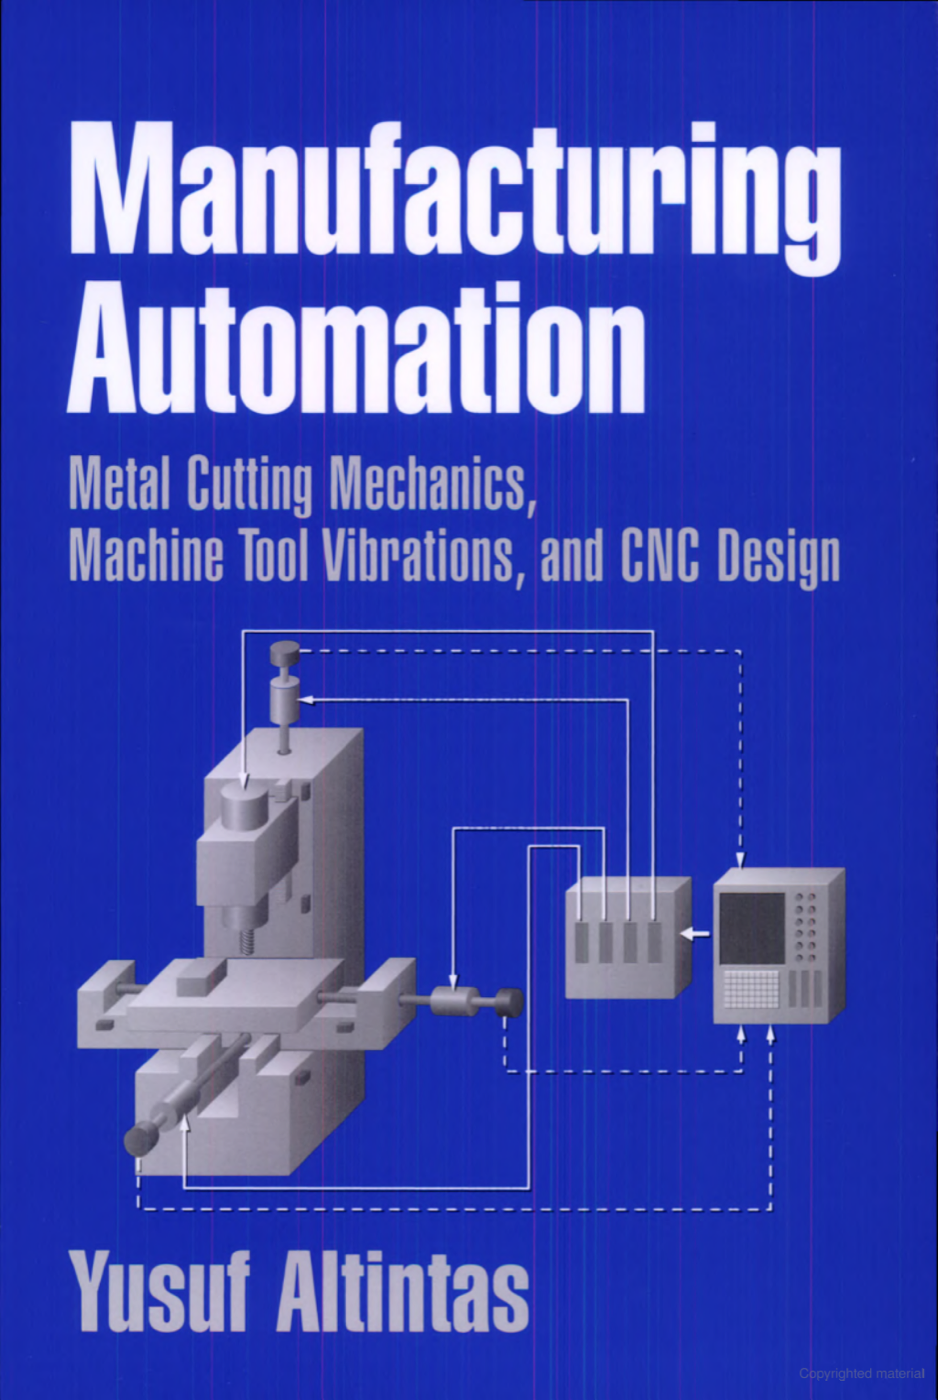
\includegraphics[width=\linewidth,height=5in,keepaspectratio]{images/altintas.png}

}

\caption{Reference book}

\end{figure}%

\section{Exam rules}\label{exam-rules}

\subsection{Normal exam}\label{normal-exam}

\begin{itemize}
\tightlist
\item
  Each Session is made up by a mandatory written exam and an optional
  oral exam

  \begin{itemize}
  \tightlist
  \item
    \textbf{Written exam:} on Moodle platform, max 26/30
  \item
    \textbf{Oral exam:} optional, max 30L/30, must be given in the same
    session
  \end{itemize}
\item
  \textbf{Final mark:} starting from written mark, oral exam can improve
  or degrade it
\end{itemize}

\subsection{Alternative: personal
project}\label{alternative-personal-project}

\begin{itemize}
\tightlist
\item
  The students extend the CNC kernel developed in class to implement a
  selection of new features, and demonstrate it on a simulated machine
\item
  The project is evaluated by the teacher and the final mark is given as
  a single oral exam (max 30L/30)
\item
  Personal projects begin \textbf{after the course end}
\end{itemize}




\end{document}
